\documentclass[prb,preprint]{revtex4-1} 
\raggedbottom
\usepackage{amsmath}
\usepackage{amsfonts}
\usepackage{graphicx}

\begin{document}

\section{Mass Spectroscopy Results and Analysis}

We conducted an experiment to determine the amount of $O_2$ used during the respiratory process. To accomplish this we normalized and subtracted background pressures from data gathered on atmospheric air and alveolar (or expired) air with observed residual populations of hydrogen and an unknown compound with 33 amu (possibly (CH$_3$OH)H$^+$ or other Volatile Organic Compounds \cite{orgs}) found in the pumping chamber during both measurements. In theory nitrogen could potentially be used to normalize the data since nitrogen is, for the most part, not consumed during respiration, however this was not found to be an accurate normalizing element. This may have been due to to an increased presence of CO$_2$ and thus the fractionalized components CO and O following respiration. However this is unlikely given that the H-O bonding energy is nearly twice that of O=O bonds who's fractionalized populations were found to be approximately 2/3 O$_2$ and 1/3 O. Thus given that CO$_2$ only makes up about 4\% of alveolar air and a contribution which is nearly 100 times less in unexpired air, the probability that fractionalized CO$_2$ was affecting this normalization is very slim \cite{comp}.

Using the residual hydrogen and the compound with 33 amu to normalize, it was found that the relative decrease in oxygen content through respiration averaged 80.10$\pm0.02\%$ between both O and O$_2$ populations, where the two unexpectedly deviated from each other by about 20\% with O$_2$ being higher. Though using the residual hydrogen and the compound with 33 amu to normalize produced a reasonably comparable value to the known 75.3\% decrease in oxygen content through respiration, other expectations were never met; the significant difference in O to O$_2$ populations, along with negligible increases in CO$_2$ and H$_2$O content where the expectations were increases by factors of approximately 90 and 12 respectively suggest something else is at play \cite{comp}. One could argue that recombined O molecules from fractionalized H$_2$O may have contributed to O$_2$'s unexpected deviation from the O population decrease, however the possibility of uncombined O from H$_2$O playing a role in, along with the fact that the increase in H$_2$O through respirations was observed to be negligible makes his seem implausible. In the end failure of this experiment to meet expectations can be summed up by a lack of experience with the mechanism. In order to conduct this experiment it would have required that the input pressure be the same for all measurements, instead the pressure inside the chamber was kept the same using the Bayard-Alpert ionization gauge. Thus our results from this experiment are likely null. Despite all this our results for the relative difference between unexpired air and alveolar air are shown in Fig \ref{asd} below.

\begin{figure}[h]
	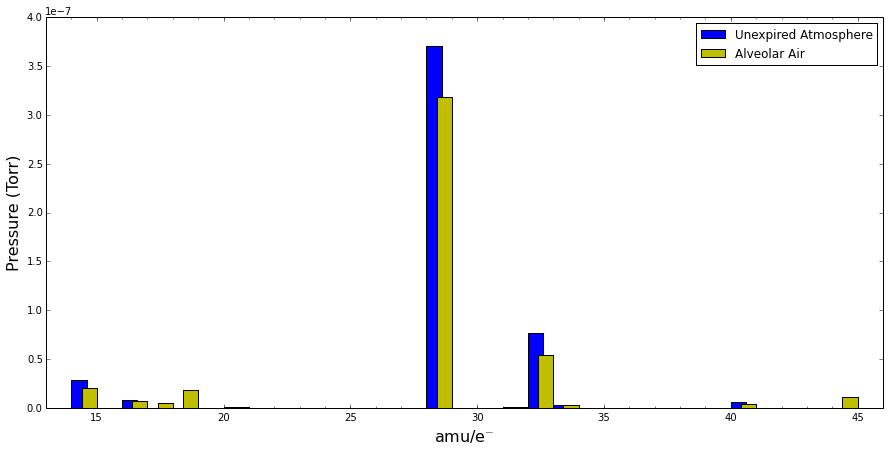
\includegraphics[width=\textwidth]{figures/Atm_Bre.png}
	\caption{The relative difference between unexpired air and alveolar air.}
	\label{asd}
\end{figure}

\newpage

\section{In Retrospect}

Only at the end of the experiment did I realize what each of the pressure gauges actually referred to. In light of that knowledge I would have liked to examine the detection efficiency of the Spectrometer. After some reading it appears that the operation and thus the efficiency of the turbo pump used in this experiment can be modeled very simply using the concept of elastic collisions. When a molecule encounters one of the fast moving blades momentum will be transferred to the molecule such that the it will leave with its velocity vector reversed while obtaining an additional component which is equal to the velocity of the blade. So if we assume the the molecules velocity is normal to the blade initially, then the resulting velocity of a molecule with an initial velocity $v_m$ which is incident on a blade with velocity $v_b$ will be $v_m+2v_b$ . The pumping rate for a particular gas should then be directly related to the fractional increase in its momentum as a result of colliding with the blade. Accordingly, the pumping rate should be proportional to $2v_b/v_m$. By considering that $v_m$ is largely related to the thermal conditions in the pump, we can say that $v_m\cong\sqrt{(2kT/m)}$ where $m$ is the mass of the molecule. This tells us that the pump efficiency should be $\propto \sqrt{m}$.

Then, using the leak valve to set a constant and arbitrary pressure inside the chamber for each element on trial, the model of efficiency could be compared to measurements of each element's pressure. We could then measure the concentration of the elements in the chamber as a function of time after closing the gate valve. Fitting an exponential to these concentration curves would produce a time constant which would be directly proportional to $m^{1/2}$. Depending on the limitations of our spectrometer this may not be possible, however, if it has the capability to measure concentration as a function of time this would be a very interesting experiment to run.

\newpage

\begin{thebibliography}{99}

\bibitem{orbs} Gouw, Joost. ``Measurement of Volatile Organic Compounds in the Earth's Atmosphere Using Proton-Transfer-Reaction Mass Spectroscopy." Mass Spectrometry Review 26 (2007): \textbf{223-257}.

\bibitem{comp} Khurana, Indu, ``Textbook of Medical Physiology'', Sanat Printers, first edition 2006, (pp. 431)

\end{thebibliography}

\end{document}